\documentclass[11pt]{article}
\usepackage[margin=1in]{geometry}
\usepackage[utf8]{inputenc}
\usepackage[T1]{fontenc}
\usepackage{lmodern}
\usepackage{amsmath,amssymb,amsthm}
\usepackage{booktabs}
\usepackage{tikz}
\DeclareUnicodeCharacter{2200}{\ensuremath{\forall}}
\DeclareUnicodeCharacter{2203}{\ensuremath{\exists}}
\DeclareUnicodeCharacter{2192}{\ensuremath{\to}}
\DeclareUnicodeCharacter{2260}{\ensuremath{\neq}}
\DeclareUnicodeCharacter{2264}{\ensuremath{\le}}
\DeclareUnicodeCharacter{2209}{\ensuremath{\notin}}
\DeclareUnicodeCharacter{2227}{\ensuremath{\wedge}}
\usepackage[title]{appendix}
\usepackage[colorlinks=true,linkcolor=blue,citecolor=blue,urlcolor=blue,pdfauthor={P. Graham},pdftitle={Combinatorial periods of asymmetric billiard trajectories in the regular pentagon}]{hyperref}
\newtheorem{theorem}{Theorem}[section]
\newtheorem{proposition}[theorem]{Proposition}
\newtheorem{corollary}[theorem]{Corollary}
\newtheorem{lemma}[theorem]{Lemma}
\newtheorem{conjecture}[theorem]{Conjecture}
\theoremstyle{definition}
\newtheorem{definition}[theorem]{Definition}
\theoremstyle{remark}
\newtheorem{remark}[theorem]{Remark}
\newtheorem{example}[theorem]{Example}
\setlength{\emergencystretch}{3em}
\newcommand{\Gp}{\Gamma^{+}}
\title{Combinatorial periods of asymmetric billiard trajectories in the regular pentagon}
\author{P. Graham\\ \small\url{https://orcid.org/0009-0007-8493-1505}}
\date{November 10, 2026}
\begin{document}
\maketitle
\begin{abstract}
We prove that every even integer other than $2$, $12$, $14$ and $18$ is
the combinatorial period, the number of bounces before repeating, of a
periodic billiard trajectory in the regular pentagon that does not have
five-fold rotational symmetry. Davis and Lelièvre conjectured this in 2018
and checked it up to period $4000$, and Kontorovich and Zhang proved it for
almost every even number. As they explain, a theorem of Davis, Fuchs and
Tabachnikov turns the question into one about vectors. Each vector
$(a+b\varphi,c+d\varphi)$ obtained from $(0,1)$ by products of four
explicit $2\times2$ matrices, where $\varphi$ is the golden ratio and
$a,b,c,d$ are integers, has the half-period $\ell=a+b+c+d$, and when a
congruence modulo $5$ holds it gives such a trajectory of period
$n=2\ell$. Varying the power of one of the two triangular matrices in such
a product gives half-periods in an arithmetic progression. We give $379$
of these progressions, which together contain every half-period $\ell\ge2$
except nine values. Six of the nine come from explicit trajectories
checked in exact arithmetic; the other three are halves of excluded
periods. The covering argument is checked in Lean, assuming the cited
theorem. Whether the four excluded periods occur is not treated.

This work has not yet been reviewed by experts.
The proofs, the Lean formalization and the text were produced by AI models
(from OpenAI and Anthropic), working under the author's direction.
\end{abstract}
\medskip
\noindent\textit{Keywords:} polygonal billiards, regular pentagon,
periodic trajectories, golden L, Hecke group, thin orbits.

\noindent\textit{MSC 2020:} 37C83, 37E35, 11B25.

\section{Introduction}

\subsection{Main result}
A billiard trajectory in a polygon moves in straight lines and reflects off
the sides with equal angles of incidence and reflection; it is
\emph{nonsingular} if it never hits a vertex. A nonsingular trajectory is
\emph{periodic} if it returns to its initial point with its initial
direction, and its \emph{combinatorial period} is the number of
reflections in a least period, the ``number of edge crossings before
repeating'' in the words of Davis and Lelièvre \cite[\S1]{DL}. Kontorovich and Zhang
call a trajectory \emph{symmetric} when it has $5$-fold rotational
symmetry \cite[\S1]{KZ}: the rotation $R$ by $2\pi/5$ about the center
maps it to itself. Otherwise it is \emph{asymmetric}. Whether trajectories
are taken with or without orientation does not matter here: if $R$ mapped
a trajectory onto itself with its orientation reversed, then so would
$R^5$, the identity, since $5$ is odd.

\begin{theorem}\label{thm:main}
For every even integer $n>0$ with $n\notin\{2,12,14,18\}$, there is a
nonsingular periodic billiard trajectory in the regular pentagon whose
combinatorial period is $n$ and which does not have $5$-fold rotational
symmetry.
\end{theorem}

Whether the four excluded periods occur for asymmetric trajectories is a
separate question, which Theorem~\ref{thm:main} does not address.

\subsection{Background}
Davis and Lelièvre showed that every positive multiple of $10$ is the
combinatorial period of a rotationally symmetric trajectory
\cite[Proposition~4.2]{DL}, and wrote \cite[\S4.1]{DL}:

\begin{quote}
Based on computer evidence, we conjecture the following:
Conjecture 4.3. Every even number arises as the combinatorial period of
an asymmetric periodic billiard trajectory on the pentagon, other than 2,
12, 14 and 18. We have verified this up to period 4000.
\end{quote}

Theorem~\ref{thm:main} is the existence statement of this conjecture.
Kontorovich and Zhang restated it as their Conjecture~1.1
\cite[\S1]{KZ}. They proved \cite[Theorem~1.2]{KZ} that ``Conjecture~1.1
is true in density, that is, almost every even number arises'', with at
most $\ll X/(\log X)^{1/40}$ exceptions up to $X$, and showed that evenness
is the only congruence obstruction \cite[Theorem~1.4]{KZ}. They explained
why the orbital circle method does not apply here \cite[Remark~1.5]{KZ},
and that their sieve method misses $\gg X/\log X$ values
\cite[Remark~4.5]{KZ}.

\subsection{Proof overview}
Section~\ref{sec:cited} states the theorem of Davis, Fuchs and Tabachnikov
\cite[Theorem~11]{DFT} that we use, in the form of
\cite[Theorem~2.1]{KZ}. To each vector $v=(a+b\varphi,c+d\varphi)$ of an
orbit $\Lambda$ of a semigroup $\Gp$ of $2\times2$ matrices it attaches the
half-period $\ell(v)=a+b+c+d$, and when a congruence modulo $5$ holds it
gives an asymmetric trajectory of period $n=2\ell(v)$. So
Theorem~\ref{thm:main} asks for every half-period $\ell=n/2$ with
$\ell\notin\{1,6,7,9\}$. Section~\ref{sec:families} shows that
one-parameter families in $\Gp$ built on a parabolic generator give
arithmetic progressions of half-periods, and Section~\ref{sec:covering}
gives $379$ progressions that together contain every $\ell\ge2$ outside the
set
\[
E=\{4,5,6,7,9,15,21,29,51\}.
\]
Section~\ref{sec:small} treats $\ell\in\{4,5,15,21,29,51\}$, the periods
$8$, $10$, $30$, $42$, $58$ and $102$, by six explicit trajectories,
checked in exact arithmetic without the cited theorem. The remaining
values $\ell\in\{1,6,7,9\}$ are the half-periods of the excluded periods.
The new step is the covering: each family gives all large members of one
residue class, so finitely many families whose classes exhaust the
residues modulo a fixed number, with the few small values checked
separately, give every half-period at once. The arithmetic of
Sections~\ref{sec:families} and~\ref{sec:covering} is checked in Lean
(Section~\ref{sec:verification}).
\section{The cited theorem}\label{sec:cited}

Let $\varphi=(1+\sqrt5)/2$, and let $\Gp$ be the semigroup generated by
\[
A=\begin{pmatrix}1&\varphi\\0&1\end{pmatrix},\quad
B=\begin{pmatrix}1&0\\\varphi&1\end{pmatrix},\quad
C=\begin{pmatrix}\varphi&\varphi\\1&\varphi\end{pmatrix},\quad
D=\begin{pmatrix}\varphi&1\\\varphi&\varphi\end{pmatrix},
\]
as in \cite[\S2]{KZ}. All entries of the generators lie in
$\mathbb{Z}_{\ge0}[\varphi]=\{p+q\varphi: p,q\in\mathbb{Z}_{\ge0}\}$, so
every vector of the orbit $\Lambda=\Gp\cdot(0,1)^t$ has the form
$v=(a+b\varphi,\,c+d\varphi)$ with $a,b,c,d\ge0$ integers, uniquely
determined since $\varphi$ is irrational. Put
\[
\ell(v)=a+b+c+d,\qquad \lambda(v)=(d-b)+2(c-a).
\]
Both are $\mathbb{Z}$-linear in $(a,b,c,d)$; we call $\ell(v)$ the
\emph{half-period} of $v$.

The geometry behind the cited theorem is as follows; the proof uses only
its consequence, Corollary~\ref{cor:period}. Billiard trajectories in the
pentagon correspond to straight lines on the double pentagon, a
translation surface made of two copies of the pentagon, by the usual
unfolding. Cutting and translating pieces of the double pentagon and
applying a linear map, operations that preserve straight lines, gives
another translation surface, the golden L \cite[\S2, Figure~2]{KZ}. A
\emph{saddle connection} on such a surface is a straight segment that
starts and ends at singular points, which come from the vertices of the
pentagons, and passes through none in between; it is recorded by its
displacement vector in the plane. A direction is \emph{periodic} when the
straight lines in it are closed, apart from those that meet a singular
point. In each periodic direction, Kontorovich and Zhang name one saddle
connection short and one long, and all the proof needs is that every
vector of $\Lambda$ is a long one. They write \cite[\S2]{KZ}:
``Each periodic direction in the golden L has a short and long saddle
connection, and all long saddle connections with directions in the first
quadrant are given by $\Lambda_L=\Gamma^+\cdot(0,1)^t$.'' They then state:

\begin{theorem}[{\cite[Theorem~2.1]{KZ}, citing \cite[Theorem~11]{DFT}}]\label{thm:dft}
``Given a long saddle connection $(a+b\varphi,c+d\varphi)\in\Gamma^+\cdot(0,1)^t$
in the golden L, let $\ell=a+b+c+d$. The combinatorial period of the
corresponding pentagon billiard trajectory is given either by $L=2\ell$ or
$L=10\ell$, depending on whether $(d-b)+2(c-a)\equiv0\pmod5$ or not
(resp.), and corresponding to whether the associated trajectory is
asymmetric or not.''
\end{theorem}

By the sentence before it, the hypothesis of Theorem~\ref{thm:dft} holds
for every $v\in\Lambda$. We use only its first case.

\begin{corollary}\label{cor:period}
If $v\in\Lambda$ and $\lambda(v)\equiv0\pmod5$, then $2\ell(v)$ is the
combinatorial period of an asymmetric periodic billiard trajectory in the
regular pentagon.
\end{corollary}

Theorem~\ref{thm:main} therefore follows from Proposition~\ref{prop:cover}
below, on values of $\ell$, together with Proposition~\ref{prop:small} for
six small periods.

\section{Parabolic families}\label{sec:families}

Write $v\in\Lambda$ as the column $(a,b,c,d)\in\mathbb{Z}_{\ge0}^4$. Using
$\varphi^2=\varphi+1$, each generator acts on these coordinates by a
nonnegative integer matrix; for example $A$ sends $(a,b,c,d)$ to
$(a+d,\,b+c+d,\,c,\,d)$. Two of the generators are parabolic:
\[
A=I+N_A,\quad N_A=\begin{pmatrix}0&\varphi\\0&0\end{pmatrix},\qquad
B=I+N_B,\quad N_B=\begin{pmatrix}0&0\\\varphi&0\end{pmatrix},
\qquad N_A^2=N_B^2=0,
\]
so $P^n=I+nN_P$ for $P\in\{A,B\}$ and all $n\ge0$.

\begin{lemma}\label{lem:family}
Let $u,w$ be words in $A,B,C,D$, let $P\in\{A,B\}$, and put
$v_n=uP^nw\cdot(0,1)^t\in\Lambda$. Then $\ell(v_n)=\ell_0+n\alpha$ and
$\lambda(v_n)=\lambda_0+n\beta$ for integers $\ell_0,\alpha,\lambda_0,\beta$,
where $\alpha=\ell(uN_Pw\cdot(0,1)^t)\ge0$. If $\alpha>0$ and
$\beta\not\equiv0\pmod5$, let $n_0\in\{0,\dots,4\}$ satisfy
$\lambda_0+n_0\beta\equiv0\pmod5$; then every $s+jm$ with $j\ge0$, where
$s=\ell_0+n_0\alpha$ and $m=5\alpha$, is $\ell(v)$ for some $v\in\Lambda$
with $\lambda(v)\equiv0\pmod5$. If $\alpha>0$, $\beta\equiv0$ and
$\lambda_0+n_0\beta\equiv0\pmod5$ for some $n_0\ge0$, the same holds with
$s=\ell_0+n_0\alpha$ and $m=\alpha$.
\end{lemma}

\begin{proof}
Since $u$ acts linearly, $v_n=uw\cdot(0,1)^t+n\,uN_Pw\cdot(0,1)^t$, and
$\ell$ and $\lambda$ are linear. The orbit vectors $v_{n_0+5j}$, or
$v_{n_0+j}$ when $\beta\equiv0$, have $\lambda\equiv0\pmod5$ and
$\ell=s+jm$.
\end{proof}

\begin{example}
Take $u$ and $w$ empty and $P=A$. Then $A^n(0,1)^t=(n\varphi,1)^t$, so
$(a,b,c,d)=(0,n,1,0)$, $\ell=n+1$ and $\lambda=2-n$. With $n=2+5j$ we get
asymmetric vectors with $\ell=3+5j$, so every $2\ell$ with
$\ell\equiv3\pmod5$ and $\ell\ge3$ is an asymmetric period.
\end{example}

A single family covers one residue class modulo its $m$, from its start
$s$ on. Kontorovich and Zhang's proof of their density theorem also
produces periods from products of parabolic powers, the vectors obtained
from $B^mA^nB^k$ \cite[(4.1)]{KZ}, with exponents restricted to progressions modulo $5$ so that
the trajectories stay asymmetric \cite[\S4]{KZ}; there $\ell$ is cubic in
the exponents, and a sieve gives almost all values. Here only one exponent
varies, so $\ell$ is linear in it, and the question becomes one of covering
residue classes.

\section{The covering}\label{sec:covering}

\begin{proposition}\label{prop:cover}
For every integer $\ell\ge2$ with $\ell\notin E$, there is $v\in\Lambda$
with $\ell(v)=\ell$ and $\lambda(v)\equiv0\pmod5$.
\end{proposition}

The proof is a finite verification organized as a tree. Let
\[
M=154\,954\,800=2^4\cdot3^2\cdot5^2\cdot7\cdot11\cdot13\cdot43,
\]
and fix the order of its prime factors
$(p_1,\dots,p_{12})=(5,5,2,3,2,7,2,3,2,11,13,43)$. A \emph{node} is a pair
$(Q,r)$ with $Q=p_1\cdots p_k$ for some $0\le k\le12$ and $0\le r<Q$; it
stands for the residue class $r\bmod Q$. The children of $(Q,r)$ are the
$p_{k+1}$ nodes $(Qp_{k+1},\,r+Qt)$ with $0\le t<p_{k+1}$. Let
$E'=E\cup\{0,1\}$. A family $(m,s)$ from Lemma~\ref{lem:family}
\emph{closes} the node $(Q,r)$ if
\[
m\mid Q,\qquad r\equiv s\pmod m,\qquad\text{and}\qquad
s\le r\ \text{ or }\ \bigl(r\in E'\text{ and } s\le r+Q\bigr).
\]

\begin{lemma}\label{lem:leaf}
If $(m,s)$ closes $(Q,r)$, then every integer $x\ge0$ with
$x\equiv r\pmod Q$ and $x\notin E'$ satisfies $x\equiv s\pmod m$ and
$x\ge s$.
\end{lemma}

\begin{proof}
Since $m\mid Q$, $x\equiv r\equiv s\pmod m$. As $0\le r<Q$ and
$x\equiv r$, either $x=r$ or $x\ge r+Q$. If $s\le r$ then $x\ge s$. If
$r\in E'$, then $x\ne r$ because $x\notin E'$, so $x\ge r+Q\ge s$.
\end{proof}

\begin{proof}[Proof of Proposition~\ref{prop:cover}]
We give $379$ families, each given by words $u$, $w$, a parabolic
generator $P$ and an exponent $n_0$,
with $m$ up to $17\,325$, $s$ up to $16\,221$, and words $w$ of length up to $44$
and $u$ up to $7$; they are listed in the Lean source
(Section~\ref{sec:verification}). For each family the hypotheses of
Lemma~\ref{lem:family} hold, with the stated $m$ and $s$. Starting from the
root $(1,0)$, we expand a node into its children until some family closes
it. The resulting tree has $2\,825$ nodes, and every leaf is closed by one of
the families; since $M=p_1\cdots p_{12}$, every branch ends by depth $12$.
Given $\ell\ge2$ with $\ell\notin E$, follow from the root the children
containing $\ell$, the class of $\ell$ modulo $Q$ at each depth, to a leaf
$(Q,r)$. By Lemma~\ref{lem:leaf}, $\ell\equiv s\pmod m$ and $\ell\ge s$ for
the family $(m,s)$ closing it, so $\ell=s+jm$ with $j\ge0$, and
Lemma~\ref{lem:family} gives $v$.
\end{proof}

The leaf condition lets the same tree cover the small values: a residue
class whose least member lies in $E'$ needs a family starting by its second
member only. The families were found by a computer search over short words
and a greedy choice of residue classes modulo $M$.

\section{Six explicit trajectories}\label{sec:small}

Place the regular pentagon with vertices $V_k=(\cos72k^\circ,\sin72k^\circ)$,
$k=0,\dots,4$, and call the segment from $V_k$ to $V_{k+1}$ side $k$
(indices mod $5$). Write $\sigma=\sin72^\circ$.

\begin{proposition}\label{prop:small}
For each row of Table~\ref{tab:small}, the billiard trajectory starting at
the point $V_0+\tfrac1{200}(V_1-V_0)$ of side $0$ with direction
$(X,\sigma Y)$ is nonsingular and periodic, has the combinatorial period
shown, and does not have $5$-fold rotational symmetry.
\end{proposition}

\begin{table}[h]
\centering
\renewcommand{\arraystretch}{1.3}
\begin{tabular}{rll}
\toprule
period & $X$ & $Y$\\
\midrule
$8$ & $-\tfrac52-\tfrac32\sqrt5$ & $0$\\
$10$ & $-\tfrac{15}4-\tfrac74\sqrt5$ & $\tfrac52-\tfrac12\sqrt5$\\
$30$ & $-10-\tfrac{11}2\sqrt5$ & $\tfrac{15}2-\tfrac12\sqrt5$\\
$42$ & $-\tfrac{65}4-\tfrac{29}4\sqrt5$ & $\tfrac52-\tfrac52\sqrt5$\\
$58$ & $-\tfrac{85}4-\tfrac{41}4\sqrt5$ & $-\tfrac52+\tfrac52\sqrt5$\\
$102$ & $-\tfrac{155}4-\tfrac{71}4\sqrt5$ & $-\tfrac{15}2-\tfrac12\sqrt5$\\
\bottomrule
\end{tabular}
\caption{Initial directions $(X,\sigma Y)$ of the six trajectories.}
\label{tab:small}
\end{table}

\begin{figure}[tb]
\centering
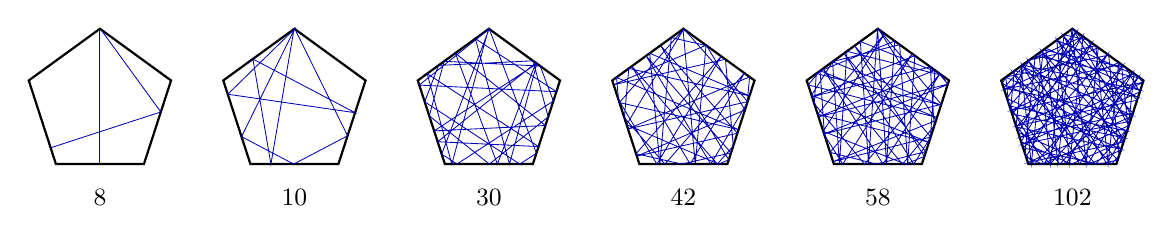
\begin{tikzpicture}[scale=0.95]
\draw[thick] (0.000,1.000) -- (-0.951,0.309) -- (-0.588,-0.809) -- (0.588,-0.809) -- (0.951,0.309) -- cycle;
\draw[blue!70!black, line width=0.3pt] (-0.005,0.997) -- (-0.005,-0.809) -- (-0.005,0.997) -- (0.012,0.991) -- (0.814,-0.112) -- (-0.659,-0.591) -- (0.814,-0.112) -- (0.012,0.991) -- cycle;
\node at (0.00,-1.25) {\small $8$};
\draw[thick] (2.600,1.000) -- (1.649,0.309) -- (2.012,-0.809) -- (3.188,-0.809) -- (3.551,0.309) -- cycle;
\draw[blue!70!black, line width=0.3pt] (2.595,0.997) -- (2.286,-0.809) -- (2.045,0.596) -- (3.411,-0.122) -- (1.709,0.125) -- (2.603,0.998) -- (1.893,-0.442) -- (2.591,-0.809) -- (3.311,-0.431) -- (2.607,0.995) -- cycle;
\node at (2.60,-1.25) {\small $10$};
\draw[thick] (5.200,1.000) -- (4.249,0.309) -- (4.612,-0.809) -- (5.788,-0.809) -- (6.151,0.309) -- cycle;
\draw[blue!70!black, line width=0.3pt] (5.195,0.997) -- (4.704,-0.809) -- (4.375,0.400) -- (5.864,-0.575) -- (4.515,-0.510) -- (5.827,0.544) -- (5.314,-0.809) -- (4.751,0.674) -- (5.955,-0.293) -- (4.468,-0.365) -- (5.841,0.534) -- (5.475,-0.809) -- (5.019,0.868) -- (6.102,0.159) -- (4.269,0.247) -- (5.203,0.998) -- (4.569,-0.675) -- (4.773,-0.809) -- (6.062,0.035) -- (5.885,0.502) -- (4.601,0.565) -- (4.403,-0.164) -- (5.206,-0.809) -- (5.993,-0.177) -- (5.790,0.572) -- (4.526,0.510) -- (4.342,0.024) -- (5.613,-0.809) -- (5.835,-0.664) -- (5.205,0.996) -- cycle;
\node at (5.20,-1.25) {\small $30$};
\draw[thick] (7.800,1.000) -- (6.849,0.309) -- (7.212,-0.809) -- (8.388,-0.809) -- (8.751,0.309) -- cycle;
\draw[blue!70!black, line width=0.3pt] (7.795,0.997) -- (7.959,-0.809) -- (8.103,0.780) -- (6.868,0.252) -- (8.362,0.592) -- (8.467,-0.566) -- (8.254,-0.809) -- (7.110,0.499) -- (7.891,-0.809) -- (8.616,0.407) -- (7.553,-0.809) -- (7.011,-0.189) -- (7.070,0.470) -- (8.684,0.103) -- (7.350,0.673) -- (7.485,-0.809) -- (7.638,0.882) -- (8.110,0.775) -- (8.623,-0.085) -- (7.178,-0.703) -- (8.522,-0.397) -- (7.494,0.778) -- (8.406,-0.752) -- (8.272,-0.809) -- (7.041,-0.282) -- (7.804,0.997) -- (6.945,0.014) -- (8.537,-0.348) -- (6.906,0.350) -- (6.933,0.051) -- (7.446,-0.809) -- (8.306,0.632) -- (7.167,-0.670) -- (7.777,-0.809) -- (8.437,-0.659) -- (7.302,0.638) -- (8.166,-0.809) -- (8.653,0.008) -- (8.685,0.357) -- (7.059,-0.339) -- (8.659,0.026) -- (7.818,0.987) -- cycle;
\node at (7.80,-1.25) {\small $42$};
\draw[thick] (10.400,1.000) -- (9.449,0.309) -- (9.812,-0.809) -- (10.988,-0.809) -- (11.351,0.309) -- cycle;
\draw[blue!70!black, line width=0.3pt] (10.395,0.997) -- (10.275,-0.809) -- (10.166,0.830) -- (11.207,0.413) -- (11.335,0.260) -- (9.607,-0.177) -- (11.163,0.446) -- (11.103,-0.454) -- (10.880,-0.809) -- (9.948,0.671) -- (11.042,-0.642) -- (10.382,-0.809) -- (9.761,-0.652) -- (10.860,0.666) -- (9.931,-0.809) -- (9.685,-0.419) -- (9.628,0.439) -- (11.190,-0.186) -- (9.468,0.250) -- (9.622,0.435) -- (10.625,0.836) -- (10.516,-0.809) -- (10.396,0.997) -- (10.415,0.989) -- (11.247,-0.010) -- (9.681,-0.406) -- (11.334,0.255) -- (11.256,0.378) -- (9.986,0.699) -- (9.886,-0.809) -- (9.794,0.560) -- (11.244,-0.020) -- (9.577,0.402) -- (9.550,-0.001) -- (10.223,-0.809) -- (11.229,0.398) -- (10.469,-0.809) -- (9.666,0.467) -- (10.729,-0.809) -- (11.153,-0.300) -- (11.101,0.491) -- (9.520,0.091) -- (10.894,0.641) -- (10.798,-0.809) -- (10.691,0.788) -- (9.797,0.562) -- (9.513,0.111) -- (11.083,-0.517) -- (9.595,-0.141) -- (10.491,0.934) -- (9.670,-0.370) -- (10.766,-0.809) -- (11.021,-0.707) -- (10.089,0.774) -- (11.106,-0.447) -- (9.802,-0.776) -- (11.177,-0.226) -- (10.410,0.993) -- cycle;
\node at (10.40,-1.25) {\small $58$};
\draw[thick] (13.000,1.000) -- (12.049,0.309) -- (12.412,-0.809) -- (13.588,-0.809) -- (13.951,0.309) -- cycle;
\draw[blue!70!black, line width=0.3pt] (12.995,0.997) -- (13.184,-0.809) -- (13.347,0.748) -- (12.088,0.189) -- (13.656,0.523) -- (13.745,-0.325) -- (13.310,-0.809) -- (12.203,0.421) -- (12.915,-0.809) -- (13.676,0.509) -- (12.492,-0.809) -- (12.367,-0.671) -- (12.504,0.640) -- (13.907,0.341) -- (13.942,0.281) -- (12.296,-0.451) -- (13.809,-0.128) -- (12.876,0.910) -- (13.689,-0.497) -- (12.987,-0.809) -- (12.315,-0.510) -- (13.133,0.904) -- (12.195,-0.139) -- (13.701,-0.460) -- (12.062,0.268) -- (12.113,0.355) -- (13.485,0.648) -- (13.625,-0.695) -- (13.522,-0.809) -- (12.332,0.515) -- (13.097,-0.809) -- (13.805,0.415) -- (12.704,-0.809) -- (12.247,-0.301) -- (12.333,0.515) -- (13.909,0.179) -- (12.644,0.741) -- (12.806,-0.809) -- (12.994,0.996) -- (13.010,0.993) -- (13.755,-0.295) -- (12.599,-0.809) -- (12.381,-0.712) -- (13.261,0.810) -- (12.251,-0.313) -- (13.652,-0.611) -- (12.128,0.066) -- (12.427,0.584) -- (13.313,0.773) -- (13.478,-0.809) -- (13.620,0.549) -- (12.179,-0.091) -- (13.943,0.285) -- (13.866,0.371) -- (12.791,0.848) -- (12.965,-0.809) -- (13.143,0.896) -- (12.407,0.569) -- (12.082,0.208) -- (13.799,-0.159) -- (12.314,0.502) -- (12.451,-0.809) -- (12.610,0.717) -- (13.713,0.482) -- (13.901,0.156) -- (12.326,-0.544) -- (13.774,-0.235) -- (12.796,0.852) -- (13.649,-0.622) -- (13.228,-0.809) -- (12.275,-0.385) -- (13.053,0.961) -- (12.160,-0.032) -- (13.731,-0.367) -- (12.110,0.353) -- (12.146,0.010) -- (12.620,-0.809) -- (13.469,0.659) -- (12.342,-0.593) -- (13.354,-0.809) -- (13.605,-0.755) -- (12.411,0.572) -- (13.210,-0.809) -- (13.884,0.358) -- (12.835,-0.809) -- (12.173,-0.073) -- (12.226,0.438) -- (13.878,0.086) -- (12.553,0.675) -- (12.708,-0.809) -- (12.888,0.919) -- (13.204,0.851) -- (13.795,-0.170) -- (12.405,-0.788) -- (13.683,-0.516) -- (12.589,0.701) -- (13.462,-0.809) -- (13.750,-0.311) -- (13.824,0.401) -- (12.247,-0.300) -- (13.865,0.045) -- (13.020,0.986) -- cycle;
\node at (13.00,-1.25) {\small $102$};
\end{tikzpicture}
\caption{The six trajectories of Proposition~\ref{prop:small}, of periods
$8$, $10$, $30$, $42$, $58$ and $102$, each starting on a side at distance
$1/200$ of the side's length from a vertex.}
\label{fig:paths}
\end{figure}

\begin{proof}
All points and directions of these trajectories have coordinates $(x,\sigma y)$
with $x,y\in\mathbb{Q}(\sqrt5)$, so each trajectory can be followed in
exact arithmetic. At each step, the next side hit is the one at the least
positive time among the sides other than the current one, the hit point is
checked not to be a vertex, and the direction is reflected in that side.
After $n$ reflections, where $n$ is the period in the table, the point,
the side and the direction are again the initial ones, and not before.
Rotation by $72^\circ$ maps the initial point and direction to a pair that
does not occur among the $n$ states of the trajectory, so the rotation does
not map the trajectory to itself. These finite computations were done by
two independently written programs, one in the coordinates above and one
in the cyclotomic field $\mathbb{Q}(\zeta_5)$ with the vertices at
$\zeta_5^k$ (Section~\ref{sec:verification}).
\end{proof}

Figure~\ref{fig:paths} shows the six trajectories. They were found in
directions of small vectors of $\Lambda$,
but Proposition~\ref{prop:small} is checked directly, without
Theorem~\ref{thm:dft}.

\begin{proof}[Proof of Theorem~\ref{thm:main}]
Let $n>0$ be even with $n\notin\{2,12,14,18\}$, and let $\ell=n/2$, so
$\ell\ge1$ and $\ell\notin\{1,6,7,9\}$. If $\ell\in\{4,5,15,21,29,51\}$,
Proposition~\ref{prop:small} gives the trajectory. Otherwise $\ell\ge2$
and $\ell\notin E$, and Proposition~\ref{prop:cover} gives $v\in\Lambda$
with $\ell(v)=\ell$ and $\lambda(v)\equiv0\pmod5$; by
Corollary~\ref{cor:period}, $n=2\ell(v)$ is the combinatorial period of an
asymmetric periodic trajectory.
\end{proof}

\section{Verification}\label{sec:verification}

The deduction of Theorem~\ref{thm:main} from Theorem~\ref{thm:dft} and
Proposition~\ref{prop:small} is checked in Lean~4 \cite{Lean}, without
external libraries. The Lean statement defines $\mathbb{Z}_{\ge0}[\varphi]$,
the generators, the orbit $\Lambda$ as an inductive predicate, $\ell$ and
the condition $\lambda\equiv0\pmod5$. Billiards are not formalized:
``some asymmetric periodic trajectory has combinatorial period $n$'' is an
opaque predicate $\mathrm{AsymPeriod}(n)$, which enters only through
Theorem~\ref{thm:dft}, stated as the axiom
\[
\forall v,\ v\in\Lambda\ \to\ \lambda(v)\equiv0\pmod5\ \to\
\mathrm{AsymPeriod}(2\ell(v)),
\]
and through the hypothesis that the six periods of
Proposition~\ref{prop:small} occur. The main formal theorem,
\texttt{dl\_conjecture\_4\_3\_existence}, says: if
$\mathrm{AsymPeriod}(n)$ holds for $n=8,10,30,42,58,102$, then it holds for
every even $n>0$ other than $2,12,14,18$. With the axiom read as
Corollary~\ref{cor:period} and the hypothesis as
Proposition~\ref{prop:small}, this is Theorem~\ref{thm:main}. Its proof
uses the axiom and Lean's standard axioms only.
Proposition~\ref{prop:cover} is the formal theorem
\texttt{long\_half\_periods}, proved with no axiom beyond Lean's standard
ones: Lemma~\ref{lem:family} and
Lemma~\ref{lem:leaf} are proved in general, and the $379$ families and the
tree of Section~\ref{sec:covering} are checked by the kernel's evaluation
of a decision procedure. Proposition~\ref{prop:small} is checked outside
Lean by the two exact programs, which also reject altered certificates.
Appendix~\ref{app:lean} gives the formal statements, and the accompanying
README gives the commands to reproduce both checks.

\section*{Acknowledgments}
This paper builds on the work of Diana Davis and Samuel Lelièvre, who
posed the question and computed the periods up to $4000$, and of Alex
Kontorovich and Xin Zhang, whose reformulation in terms of $\Gp$ and
statement of the period theorem are the starting point of the proof. The
period theorem is due to Diana Davis, Dmitry Fuchs and Serge Tabachnikov.

\begin{thebibliography}{9}
\bibitem{DFT}
D.~Davis, D.~Fuchs and S.~Tabachnikov,
\emph{Periodic trajectories in the regular pentagon},
Mosc. Math. J. \textbf{11} (2011), no.~3, 439--461;
\href{https://arxiv.org/abs/1102.1005}{arXiv:1102.1005}.

\bibitem{DL}
D.~Davis and S.~Lelièvre,
\emph{Periodic paths on the pentagon, double pentagon and golden L},
\href{https://arxiv.org/abs/1810.11310v2}{arXiv:1810.11310v2} (2024).

\bibitem{KZ}
A.~Kontorovich and X.~Zhang,
\emph{On the local-global conjecture for combinatorial period lengths of
closed billiards on the regular pentagon},
Int. Math. Res. Not. IMRN \textbf{2025} (2025), no.~15, rnaf227,
\href{https://doi.org/10.1093/imrn/rnaf227}{doi:10.1093/imrn/rnaf227};
\href{https://arxiv.org/abs/2409.10682}{arXiv:2409.10682}.

\bibitem{Lean}
L.~de~Moura and S.~Ullrich,
\emph{The Lean 4 theorem prover and programming language},
in: Automated Deduction -- CADE 28, Lecture Notes in Comput. Sci.
\textbf{12699}, Springer, 2021, 625--635.
\end{thebibliography}

\begin{appendices}
\section{The formal statements}\label{app:lean}

The definitions are in \texttt{Pentagon/Statement.lean}. An element
$p+q\varphi$ of $\mathbb{Z}_{\ge0}[\varphi]$ is a pair of natural numbers
with the product $(p+q\varphi)(r+s\varphi)=pr+qs+(ps+qr+qs)\varphi$; a
vector is a pair of these and a matrix a quadruple. The generators are
\texttt{A}, \texttt{B}, \texttt{C}, \texttt{D}, written entrywise as in
Section~\ref{sec:cited}. \texttt{Orbit v} is the least predicate
containing $(0,1)$ and closed under the four generators; \texttt{ell v} is
$a+b+c+d$ and \texttt{Asym v} is $((d-b)+2(c-a))\bmod 5=0$ in the
integers. The cited theorem is the axiom
\begin{verbatim}
axiom kz_thm_2_1 : ∀ v : Vec, Orbit v → Asym v → AsymPeriod (2 * ell v)
\end{verbatim}
whose documentation quotes Theorem~\ref{thm:dft} and the sentence before
it. The main theorem, in \texttt{Pentagon/Proof.lean}, is
\begin{verbatim}
theorem dl_conjecture_4_3_existence
    (small : AsymPeriod 8 ∧ AsymPeriod 10 ∧ AsymPeriod 30 ∧
      AsymPeriod 42 ∧ AsymPeriod 58 ∧ AsymPeriod 102) :
    ∀ n : Nat, 0 < n → n % 2 = 0 → n ≠ 2 → n ≠ 12 → n ≠ 14 → n ≠ 18 →
      AsymPeriod n
\end{verbatim}
and Proposition~\ref{prop:cover} is
\begin{verbatim}
theorem long_half_periods (l : Nat) (h2 : 2 ≤ l) (hl : l ∉ exceptions) :
    ∃ v, Orbit v ∧ ell v = l ∧ Asym v
\end{verbatim}
with \texttt{exceptions} the list $4,5,6,7,9,15,21,29,51$. The file
\texttt{Pentagon/Cert.lean} lists the $379$ families by the depth of the
nodes they close, each as $(m,s,w,P,u,n_0)$, and the prime order.
\texttt{famOK} checks a family against Lemma~\ref{lem:family} by computing
$uw\cdot(0,1)^t$ and $uN_Pw\cdot(0,1)^t$, and \texttt{chk} walks the tree,
expanding a node until \texttt{leafOK}, the closing condition, holds; both
are evaluated by the kernel (\texttt{decide +kernel}), and their soundness
lemmas \texttt{fam\_sound}, \texttt{leaf\_sound} and \texttt{chk\_sound} are
proved. The build file \texttt{PublicChecks.lean} restates these theorems with
their full types and checks their axioms: \texttt{long\_half\_periods}
uses only the standard axioms of Lean's logic, and
\texttt{dl\_conjecture\_4\_3\_existence} uses these and the cited axiom. The development also proves
\texttt{exceptions\_combinatorial}: no $v\in\Lambda$ with
$\lambda(v)\equiv0\pmod5$ has $\ell(v)$ or $\ell(\varphi v)$ in
$\{1,6,7,9\}$, a statement about the orbit that Theorem~\ref{thm:main}
does not use.
\end{appendices}
\end{document}
